% **************************************************
%   Wichtig für die verwendung der hsrmreport-Klasse!
%   
%   Die Datei hsrmreport.cls muss in dem selben Ordner sein
%   wie die .tex Datei die diese Klasse verwenden möchte.
%
%   Desweiteren ist die Dokumentenklasse nach aktuellem 
%   noch ohnen Optionen, sprich Zweiseitig, änderung 
%   der Schriftgröße oder ähnliches. Ich werde versuchen 
%   diese Features hinzu zufügen sobald es mir möglich ist. 
%
%   Falls Ihr Probleme, Anregungen oder Verbesserungen habt,
%   könnt ihr mir das gerne mitteilenen.
%
%   Es kann sein das ihr evtl. manche Packete noch installieren 
%   müsst bevor die Klasse Fehlerfrei funktioniert.
%   Meldungen wie "Command terminated with space." können ignoriert werden.
%
%   Ich werde auch eine Übersicht aller Pakete schreiben, die ich verwendet habe.
%      
%
%   E-Mail: timjonas.wechler@student.hs-rm.de
% **************************************************


\documentclass{hsrmreport}
% **************************************************
% Ihr könnte die Angaben der TITELSEITE hier ändern
% **************************************************
\newcommand{\titel}{Abschlussaufgabe}
\newcommand{\studiengang}{Angewandte Pyhsik}
\newcommand{\studienrichtung}{}
\newcommand{\dokumentenart}{Praktikumsbericht}
\newcommand{\kurs}{LV:\ Messdatenerfassung}
\newcommand{\versuchsdurchfuehrung}{10. Februar 2021}

%Falls ihr weniger als vier Studenten seit könnt ihr dies Einträge die zu viel sind einfach löschen. 
%Ein Feature für das angeben der Mat.Nr. ist noch in Arbeit. 
\newcommand{\studentA}{Pfitzner, Moritz}
\newcommand{\matStudentA}{(XXXXXXX)}
\newcommand{\studentB}{Wechler, Tim-Jonas}
\newcommand{\matStudentB}{(1137877)}
\newcommand{\studentC}{}
\newcommand{\matStudentC}{}
\newcommand{\studentD}{}
\newcommand{\matStudentD}{}


% Mit dem Befehl \today wird immer das aktuelle Datum auf der Titelseite ausgebeben.
% Wenn dies nicht erwünscht ist einfach manuell das gewünschte Datum eintragen.
\newcommand{\datum}{\today}



\begin{document}
    % **************************************************
    %
    %   ALLES zwischen hier und dem Begin des Berichts 
    %   nicht ändern, außer ihr wisst was ihr tut ;). 
    %
    % **************************************************

    % Title 
    \frontpage

    %Römischen Seitenzahl
    \pagenumbering{Roman}
    
    %Inhaltsverzeichnis
    \tableofcontents

    %Abbildungsverzeichnis
    \listoffigures

    %Tabellenverzeichnis
    \listoftables

    
    \clearpage

    %Normale Seitenzahlen
    \pagenumbering{arabic}

    %Das seitenLayout mit Kapitel und Unterkapitel im Header jeder Seite des Berichts
    \pagestyle{scrheadings}

    % **************************************************
    %
    % HIER BEGINNT DER BERICHT
    %
    % **************************************************

    
        \chapter{Vorbereitung}
    \section{Aufbau eines Oszilloskop-Tastkopfes}
        Der Tastkopf dient als Verbindung zwischen dem Oszilloskop und der zu messenden Spannung. Es ist auch möglich ein Kabel zu verwenden, jedoch sind dann Widerstand und Kapazität bei der Messung undefiniert. Bei hohen Frequenzen wird dadurch das Messsignal verfälscht. Der Tastkopf kann die Spannung unter bekannten Bedingungen Messen.~\cite{tastkopf_deniz}
        Die Signalverarbeitung eines Tastkopfes kann mit passiven Bauelementen erfolgen oder durch eine aktive Schaltung. Wichtig ist das der Eingangswiderstand eines Tastkopfes möglichst groß und die Einkangskapazität möglichst klein ist, damit das Signal unverfälscht weitergegeben wird. Dabei gibt es viele verschiedene Tastköpfe mit eigenen Eigenschaften. Im Folgenden sind diese mit ihrem Aufbau aufgelistet.~\cite{tastkopf_wiki}

        \begin{enumerate}

        \item Standard-Tastkopf
            \begin{figure}[h!]
                \centering
                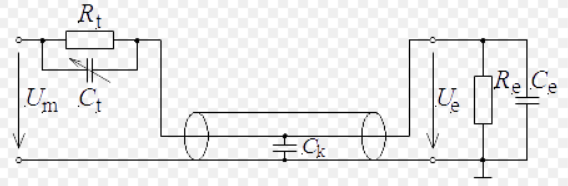
\includegraphics[]{111.PNG}
                \caption{Aufbau eines Standart Tastkopfes~\cite{tastkopf_standard}}
            \end{figure}

        \item Transmissions-Line-Tastkopf
            \begin{figure}[h!]
                \centering
                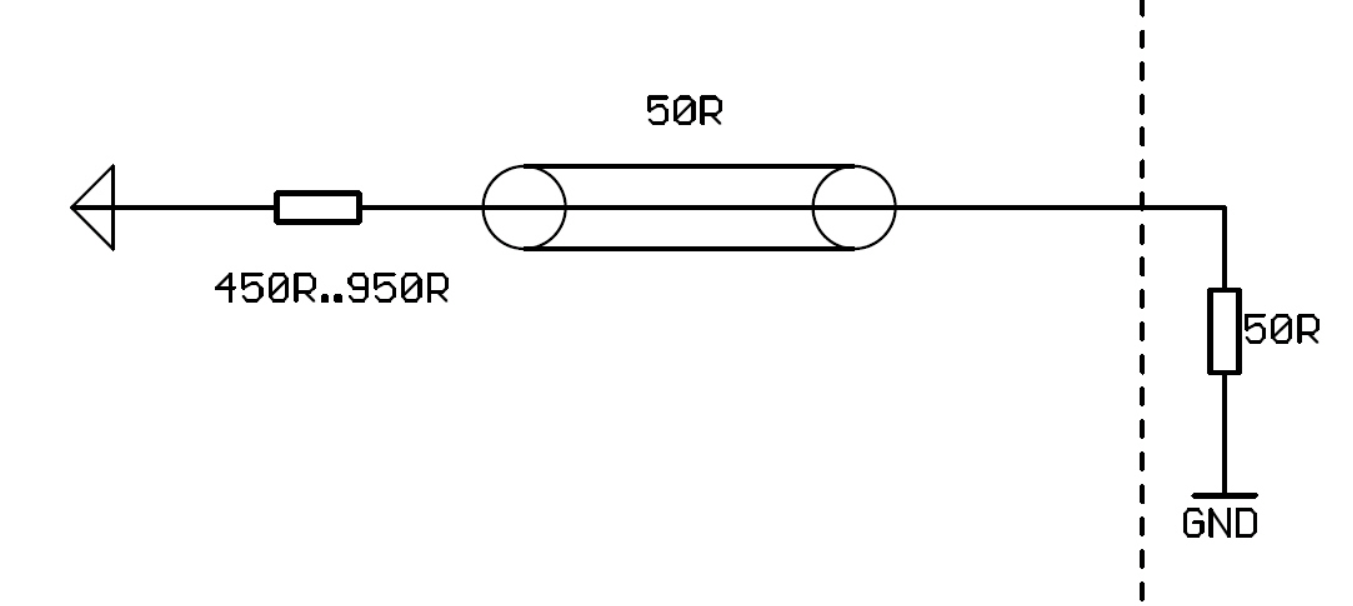
\includegraphics[width=0.5\linewidth]{112.PNG}
                \caption{Aufbau eines Transmission-Line-Tastkopfes~\cite{transmission_line_probe}}
            \end{figure}
        \newpage
        \item Aktiver Tastkopf
            \begin{figure}[h!]
                \centering
                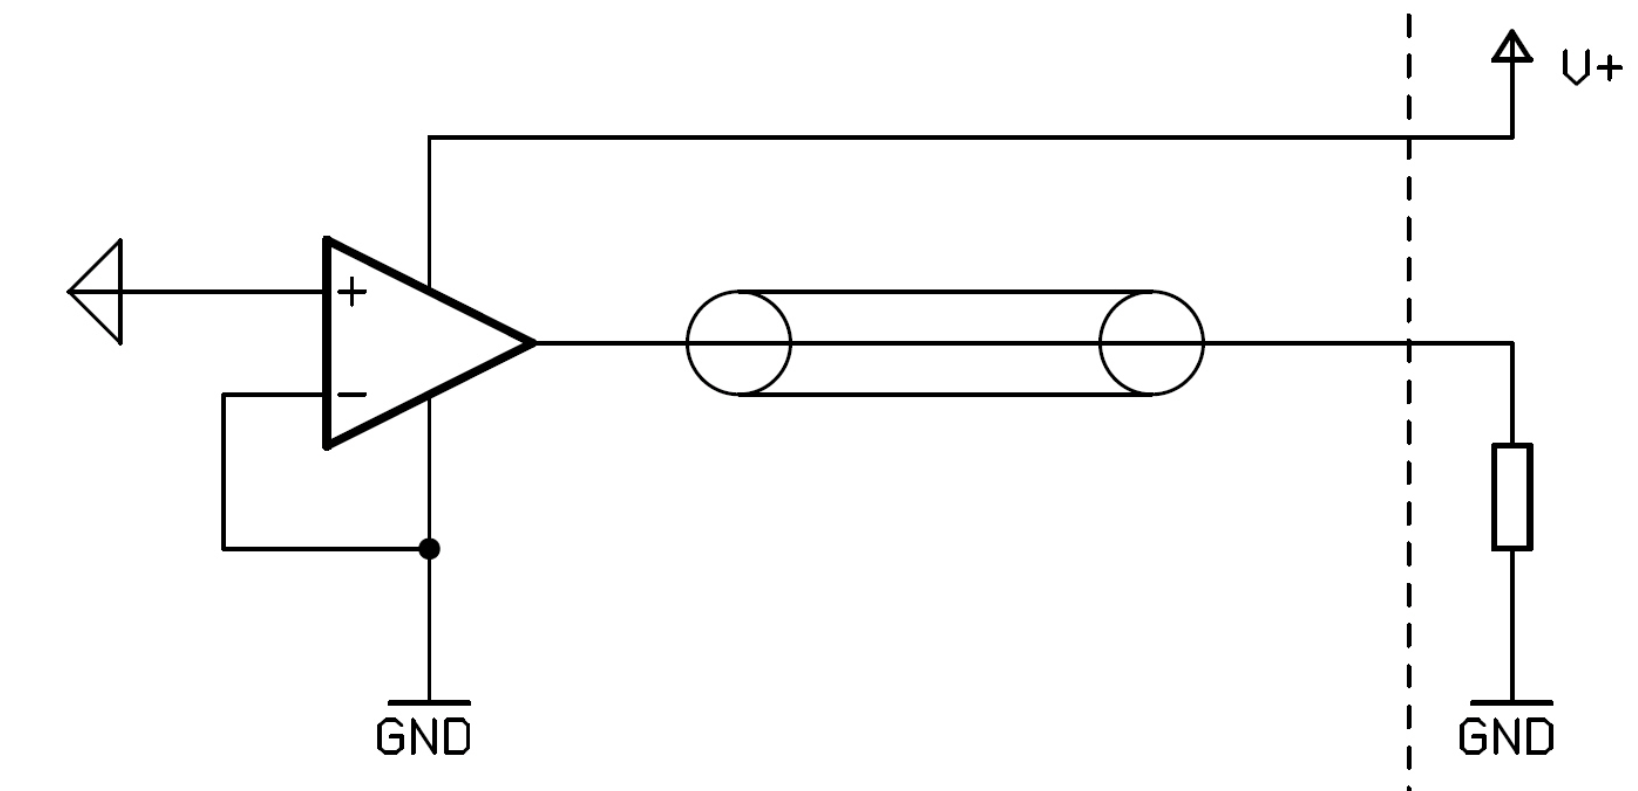
\includegraphics[width=0.5\linewidth]{113.PNG}
                \caption{Aufbau eines aktiven Tastkopfes~\cite{active_probe}}
            \end{figure}

        \item Differentieller Tastkopf
            \begin{figure}[h!]
                \centering
                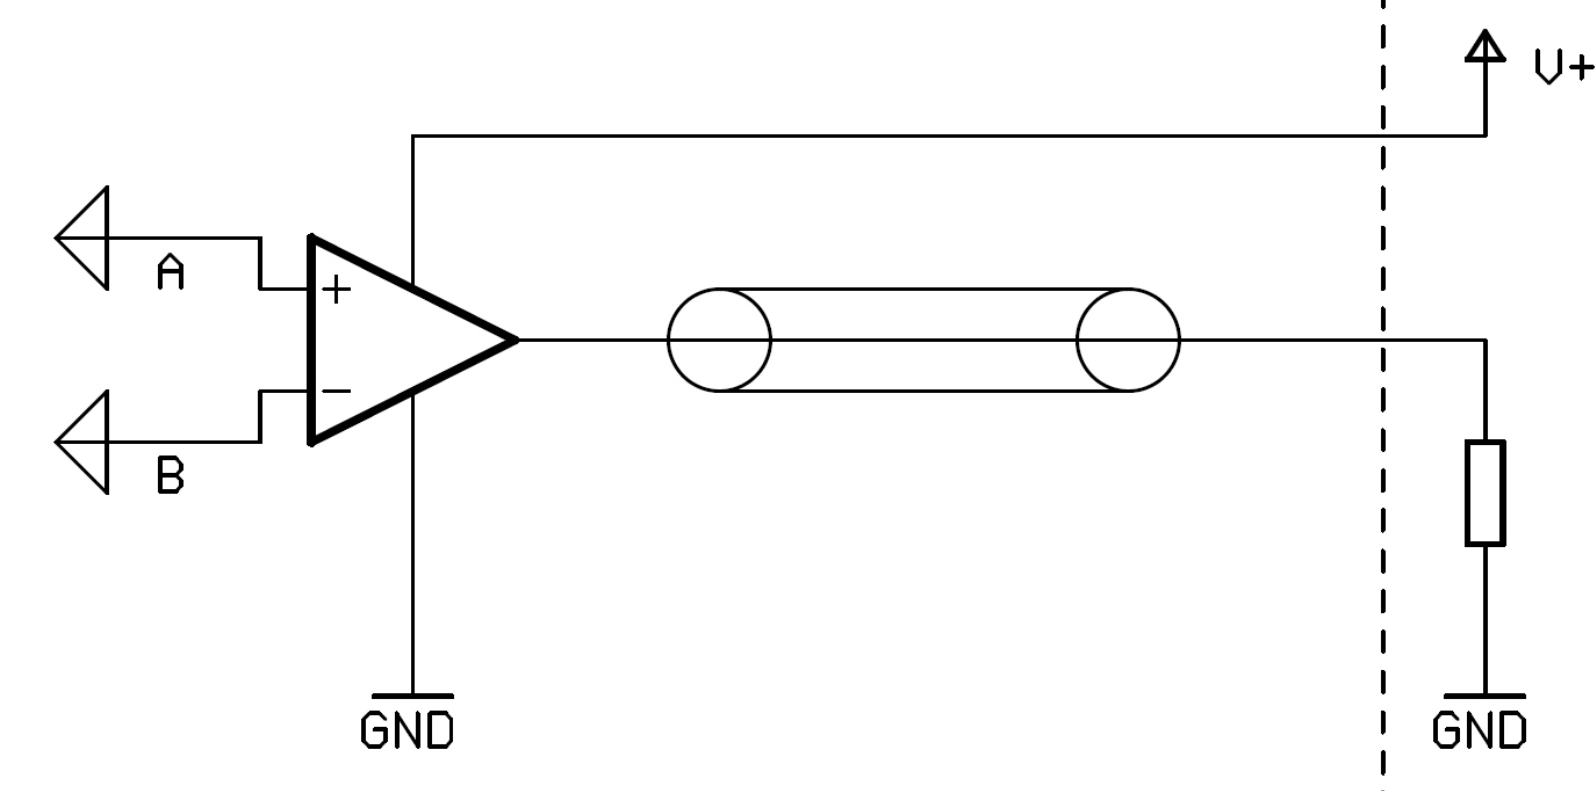
\includegraphics[width=0.5\linewidth]{114.PNG}
                \caption{Aufbau eines differentiellen Tastkopfes~\cite{differential_probe}}
            \end{figure}

        \end{enumerate}

        \begin{table}[h!]
            \centering
            \caption{Begriffserklärung für die einzelnen Buchstaben in den Abbildungen}
            \begin{tabular}{|c|c|}
                \hline
                $R_t$ & Tastkopfwiderstand\\ \hline \hline
                $C_t$ & Tastkopfkapazität \\ \hline
                $U_m$ & Spannungsmessung\\ \hline
                $C_K$ & Kabelkapazität\\ \hline
                $U_e$ & Eingangsspannung\\ \hline
                $R_e$ & Eingangswiderstand\\ \hline
                $C_e$ & Eingangskapazität\\ \hline
                Zahl mit R & Widerstand mit Zahlenwert \\ \hline
                GND & Ground (zu Erde)\\ \hline
                V & Spannung\\ \hline
            \end{tabular}
        \end{table}


        \input{content/kalibierung.tex}
        \chapter{Auswertung der Messdaten}
    \section{Kalibrierung}
        Bevor man die Werte auslesen kann muss eine Kalibrierung gemacht werden. Diese wurde von Herrn Dörr durchgeführt. In der Datei \texttt{Kalibriermessung\_3.txt} 
        befinden sich die Signalausgabe des Beschleunigungssensors während der Kalibrierung.
        Diese Werte werden in der Grafik~\ref{kaligraf} mit Hilfe von SciDAVis veranschaulicht.\\
        \begin{figure}[ht!]
            \centering
            \includegraphics[width=\linewidth]{images/kalibrierung.png}
            \caption{grafische Darstellung der Kalibrierwerte}
            \label{kaligraf}
        \end{figure}
        
        \subsection{Bestimmung des Kalibrierfaktors}
            Mit dem Courser-Tool werden die Werte \(ADC_{z1}\) und \(ADC_{z2}\) ausgelesen. 
            \begin{table}[!ht]
                \centering
                \caption{Messwerte \(ADC_{z1}\) und \(ADC_{z2}\) der Kalibrierung}
                \begin{tabular}{|c|c|}
                    \hline
                    \(ADC_{z1}\) & \(ADC_{z2}\)\\ \hline 
                    1292 & 844 \\ \hline
                \end{tabular}
                \label{kali}
            \end{table}
            Setzt man nun die Werte in die Gleichung 3 aus dem Aufgabenblatt ein, so ergibt sich folgende Rechnung.
            \begin{align*}
                k_z&=\frac{a_{z1}-a_{z2}}{ADC_{z1}-ADC_{z2}}\\
                &=\frac{2\cdot \SI{9.81}{\meter\per\square\second}}{1292-844}\\
                &=\SI{0,044}{\meter\per\square\second}
            \end{align*}
        \subsection{Bestimmung des Offset's $ADC_{z0}$}
            Um Offset \(ADC_{z0}\) bestimmen zu können werden die Werte aus der Tabelle~\ref{kali} in die Gleichung 4 aus dem Aufgabenblatt eingesetzt. 
            \begin{align*}
                ADC_{z0}&=\frac{ADC_{z1}+ADC_{z2}}{2}\\
                &=\frac{1292+844}{2}\\
                &=1068 
            \end{align*}
        \subsection{Vergleich des \(k_z\) Wert mit der Empfindlichkeit des Datenblatts}
            Die Empfindlichkeit, die im Datenblatt angegeben wird, hat mit dem \(k_z\) Wert nichts direkt zu tun. Die Empfindlichkeit bezieht sich auf die Messgenauigkeit des Sensors. 
            Der \(k_z\) Wert ist an die örtliche Gegebenheit ausgelegt. Dieser Faktor beschreibt das Verhältnis der digitalen Ausgangsgröße zu der physikalischen Größe.
    \section{Beschreibung des verwendeten Blockdiagramms} 
        Das gesamte Blockdiagram wird von einer While-Schleife umschlossen. Diese wird nach einer Ausführung für \SI{1000}{\milli\second} angehalten. 
        Ebenso befindet sich dort die Abbruchfunktion über den Stop-Button.\par
        Die Datei, mit den Messdaten, wird über ein \textbf{Path-Module} eingelesen und wird an das Modul \textbf{Tabelle auslesen} weiter gereicht. Darauf folgt die lesung der Spalten. Mit den Konstanten \textbf{0} und \textbf{3} geben wir an, dass wir aus den Messdaten die Spalte 0, mit der gemessenen Zeit und Spalte 3 mit dem Ausgangssignal in z-Richtung.
        Aus dem Datenstrom der Spalte ein lässt sich die maximale Zeilenanzahl auslese und wird an eine numerische Frontpanel-Ausgaben weiter geschleift.
        Dieser Datenstrom wird auch noch für die jeweilige Grafen als X-Wert eingebunden. \par
        Der Datenstrom der aus Aus der Spalte 3 ausgelesen wird, wird zunächst an eine Savitzky-Golay-Filter weitergeleitet mit eine Angabe von 20 Seitenpunkte.
        Im Anschluss wird der \textbf{Offset a} von dem Datenstrom subtrahiert und der \(k_z\)-Wert multipliziert. Das Ergebnis geht nun weiter an den ersten Graf und wird hier als Y-Wert eingebunden. 
        Zusätzlich wird von diesem Wert der \textbf{Offset v} subtrahiert und im Anschluss in ein Integrations Modul weitergeleitet. Für d(t) wird der Wert 0,005 dem Modul angegeben. Das Ergebnis aus diesem Mudol wird in den Graf für die Geschwindigkeit als Y-Wert eingebunden und gleichzeitig nochmals auf die selbe Weise integriert.
        Nach der zweiten Integration wird auch dieser Wert in eine Graf als Y-Wert eingebunden. Dieser Graf beschreibt die zurückgelegte Strecke.
        \begin{figure}[ht!]
            \centering
            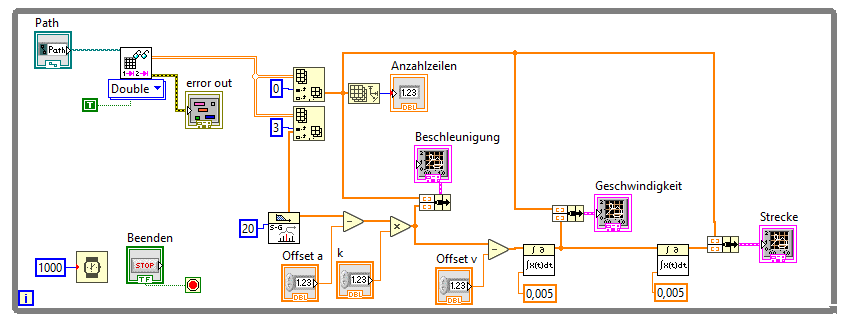
\includegraphics[width=\linewidth]{images/blockdiagramm.PNG}
            \caption{Blockdiagramm aus LabVIEW}
            \label{block}
        \end{figure}
    \section{Front Panel}
        \begin{figure}[ht!]
            \centering
            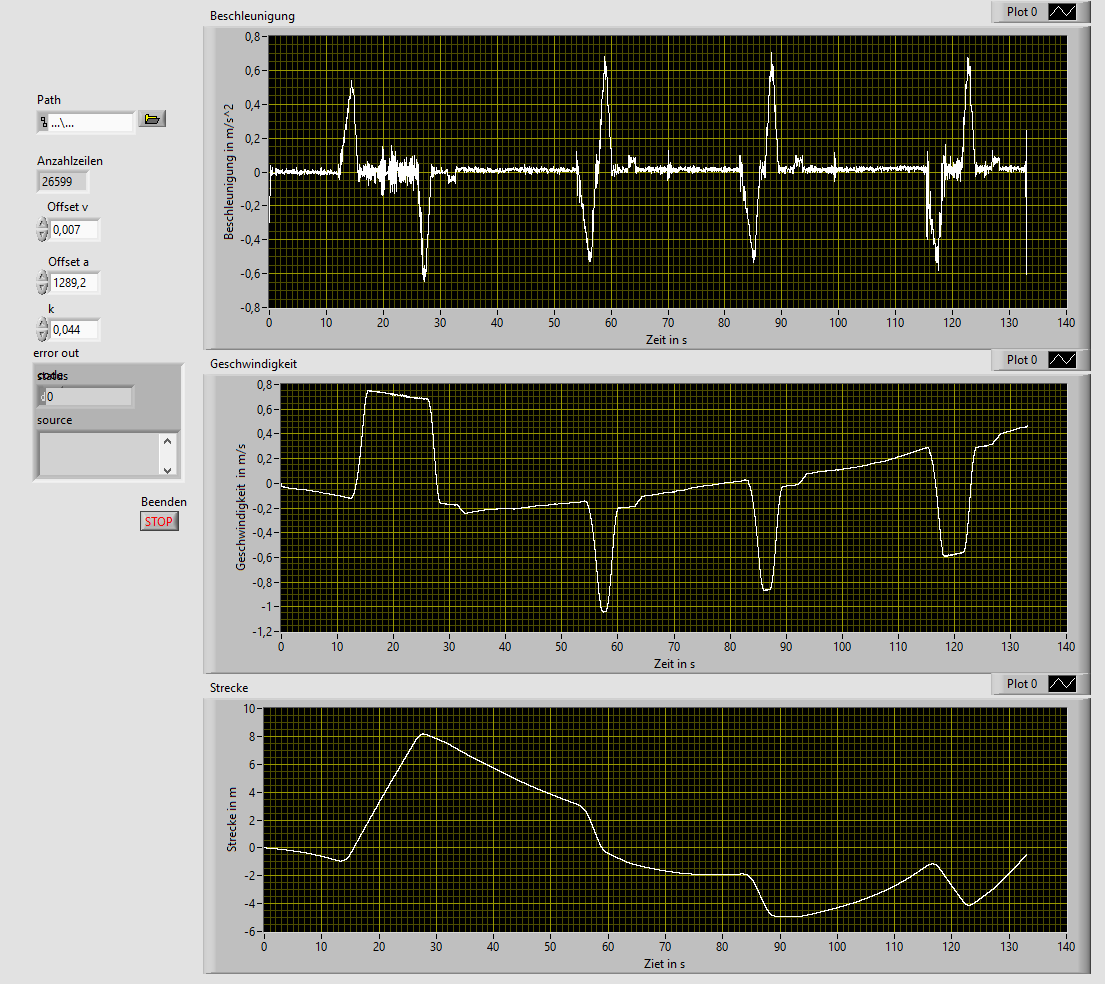
\includegraphics[width=\linewidth]{images/vi.PNG}
            \caption{VI was in LabVIEW erstellt wurde}
            \label{vi}
        \end{figure}
        
    \section{\textit{a(t)-, v(t)-, s(t)-Diagramm}}
        
        \subsection{Ermittlung des Offset's \textit{a} und \textit{v}}
            Für die Ermittlung von \textbf{Offset a} haben wir den ersten Wert aus der vierten Spalte der Messdaten abgelesen. Hier stand ein Wert von 1289. Durch ausprobieren kommen wir auf einen Wert von 1289,2  \par
            Die Ermittlung des \textbf{Offset v} ergab durch ausprobieren einen Wert von 0,007. Damit ist der Endpunkt der Strecke wieder auf der Nulllinie.
        \subsection{Ermittlung von $a_{max}$, $v_{max}$ und $s_{ges}$}
            Bei der Ermittlung der Werte für $a_{max}$, $v_{max}$ und $s_{ges}$ haben wir die jeweilige Werte aus den Abbildungen abgelesen. 
            Hierbei haben wir folgende Werte feststellen können.\par
            Für die maximale Beschleunigung haben wir einen Wert von ca. \SI{0,7}{\meter\per\square\second} ablesen können.\\
            Für die maximale Geschwindigkeit haben wir einen Wert von ca. \SI{0,9}{\meter\per\second} ermitteln können.
            Für die gesamte Strecke haben wir einen Wert von ca. \SI{9}{\meter} feststellen können.
            \begin{figure}[ht!]
                \centering
                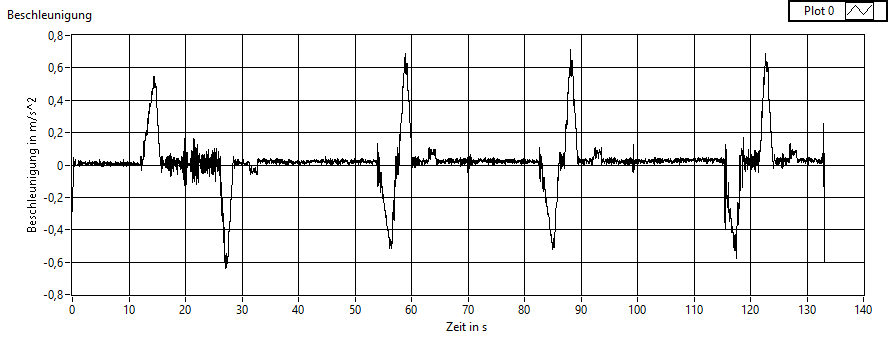
\includegraphics[width=\linewidth]{images/beschleunigung.png}
                \caption{Messwerte umgerechnet in Beschleunigung}
            \end{figure}
            \begin{figure}[ht!]
                \centering
                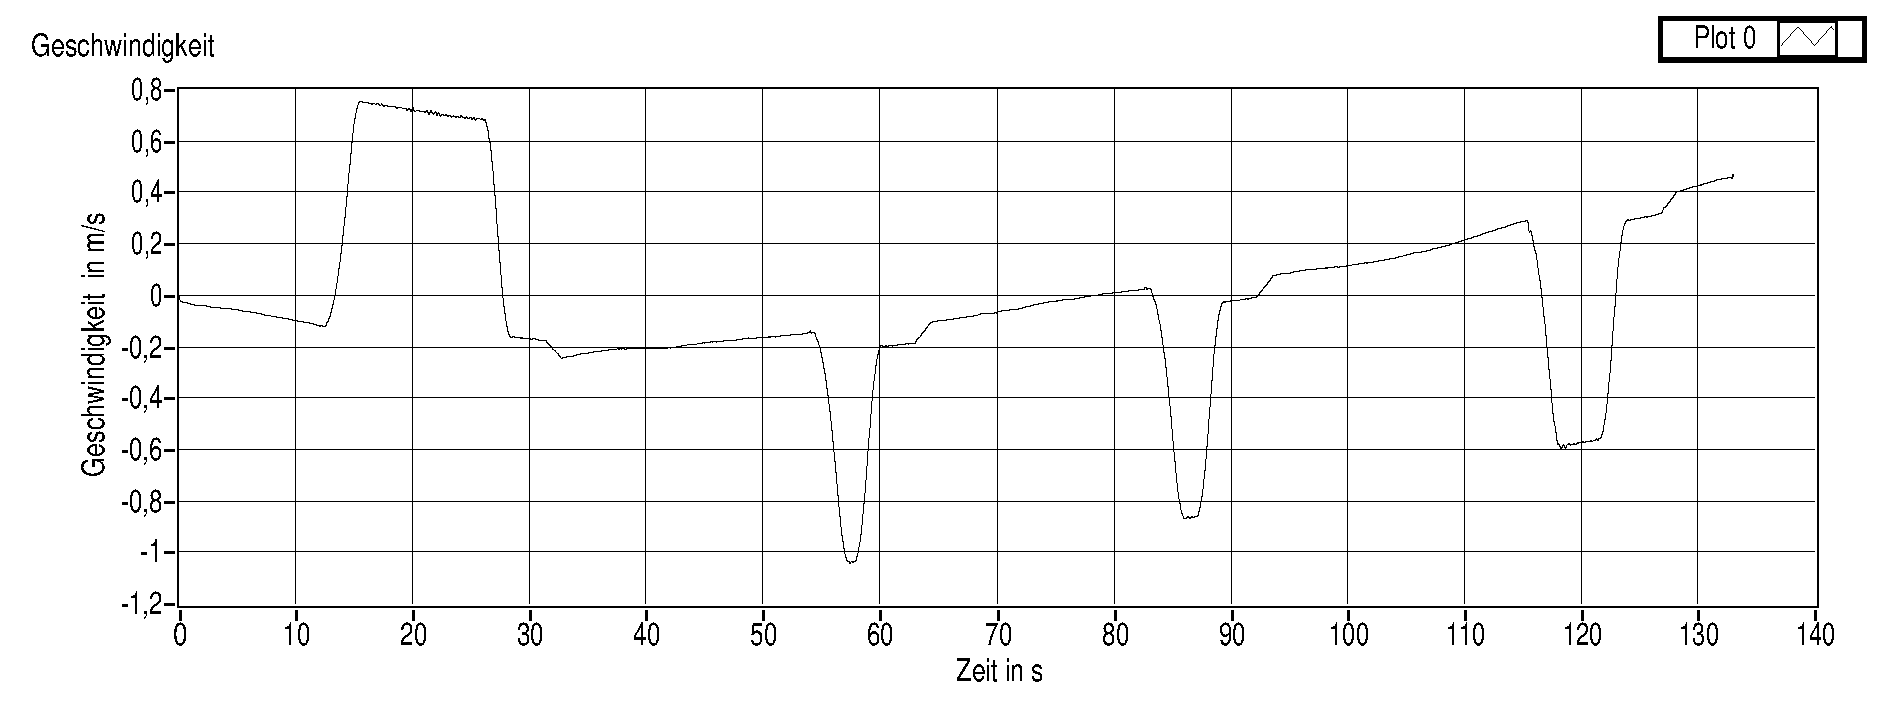
\includegraphics[width=\linewidth]{images/geschwindigkeit.eps}
                \caption{Geschwindigkeit aus den Werten der Beschleunigung integriert}
            \end{figure}
            \begin{figure}[ht!]
                \centering
                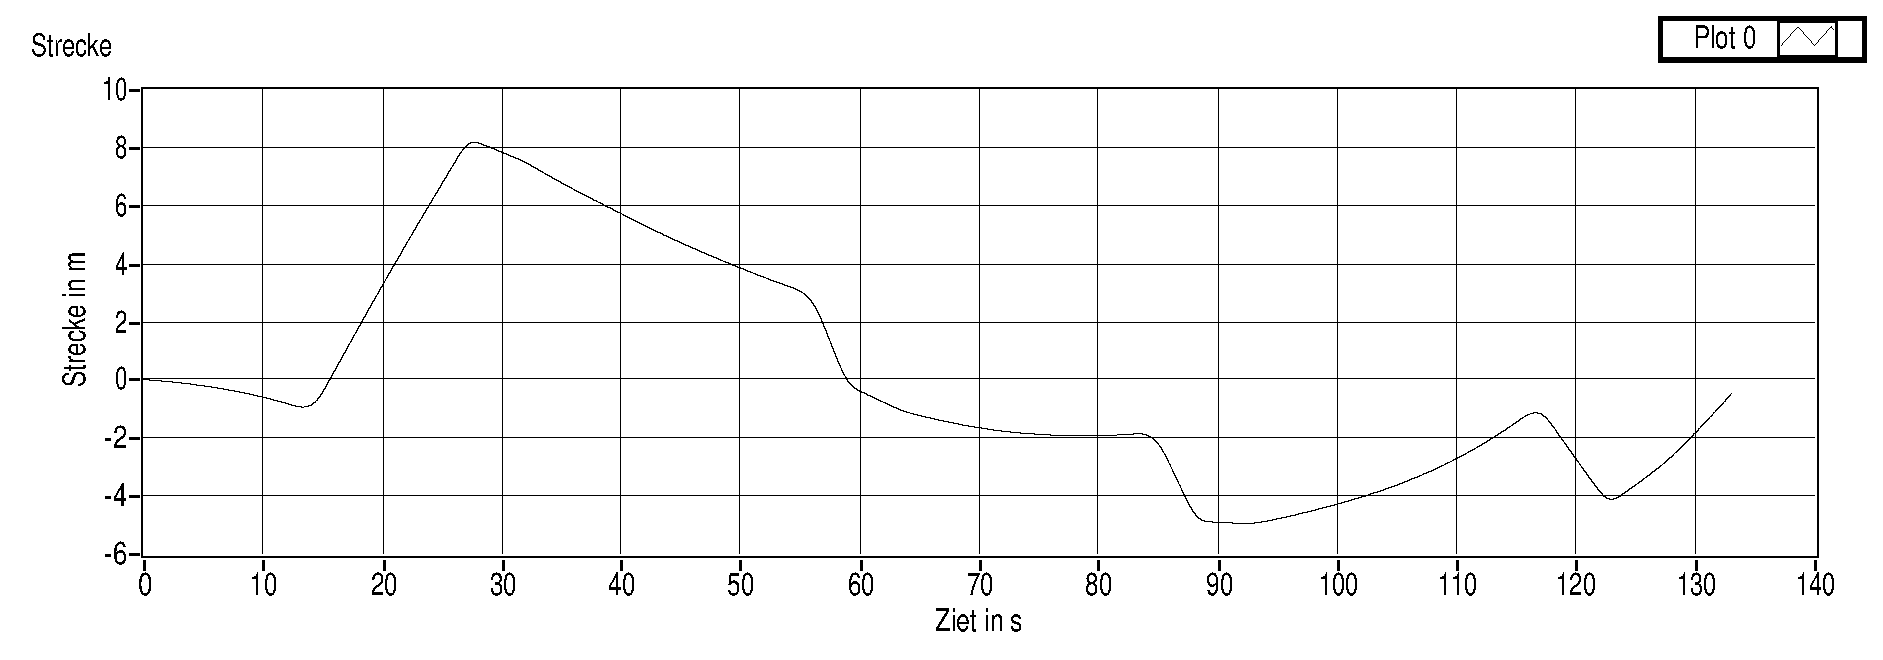
\includegraphics[width=\linewidth]{images/strecke.eps}
                \caption{Zurückgelegte Strecke aus den Werten der Geschwindigkeit integriert}
            \end{figure}
    \section{Messauflösung $a_{LSB}$}    
        Die Ermittlung des \(a_{LSB}\) haben wir mit Hilfe des \textbf{Offset a} und dem Wert der Erdbeschleunigung versucht zu berechnen.
        Hierbei sind wir wie folgt vorgegangen.
        \begin{align*}
            a_{LSB}&= \frac{g}{\textmd{Offset a}}\\
            &=\frac{\SI{9,81}{\meter\per\square\second}}{1298}\\
            &=\SI{0,008}{\meter\per\square\second}
        \end{align*}
        \chapter{Plausibilität}
    \section{Abschätzung der Messunsicherheit}
            Zur Abschätzung der Messunsicherheit haben wir die Streuung im Stillstand im Graf für die Beschleunigung betrachtet. Hieraus nehmen wir einen Wert von \SI{0,03}{\meter\per\square\second} für die Messunsicherheit an.
    \section{Vergleich der Messdaten mit reellen Daten}
        Bei der Recherche für die reellen Daten sind wir auf die Internetseite \href{http://kloke-aufzug.de/technische-daten/}{http://kloke-aufzug.de/technische-daten/} gestoßen. 
        Hier zeigt die Tabelle Technische Daten für unterschiedliche Größen von Mehrpersonenaufzügen. 
        Aus der Tabelle kann man erkennen das die meisten Aufzüge eine Geschwindigkeit von \SI{1,0}{\meter\per\second} haben, was der Messung sehr nahe kommt.

        \chapter{Fazit}
Bei dem Versuch werden erstmal die Grundlegenden Begriffe der Gleich- und Wechselspannung erklärt. 
Diese sind dann durch ein Voltmeter in die Schaltungen eingebracht worden. 
Dabei sind Schaltungen wie der Spannungsteiler und das Potentiometer aufgebaut worden 
und durch LTSpice simuliert. Zum besseren Verständnis des Graphen wurde 
dann der Effektivwert sowie die Ausgangsspannung per Hand ausgerechnet und mit den von 
LTSpice simulierten Werten verglichen. Die Werte für den Spannungsteiler und den Potentiometer
 haben mit den zu erwarteten Werten wunderbar funktioniert. Bei dem Rechtecksignal einer 
 Spannungsquelle sind jedoch zwischen simuliertem und berechneten Effektivwert Differenzen 
 aufgetreten. Ursprung des Fehlers kann in der Rechnung liegen, obwohl diese öfters zum Überprüfen 
 der Richtigkeit durchgeführt wurde. Der Fehler kann auch in der falschen Durchführung von 
 LTSpice liegen. In der Aufgabenstellung von 2.1 (Signalquellen), war nicht genau ersichtlich ob 
 das Voltmeter durch eine Wechselspannung oder Gleichspannung angetrieben wird. Durch eine 
 Wechselspannung würde der Graph von -1V bis 1V gehen. Die simulierten Graphen in dem Bericht 
 sind jedoch nur von 0V bis 1V aufgetragen. Durch die Wechselspannung sind die berechneten Werte 
 aber auch nicht zu erzielen, da diese ebenfalls zur Lösung des Problems simuliert wurden und 
 nicht mit den berechneten Werten übereinstimmen. 
    
    
    
    \printbibliography
\end{document}